% Created 2023-12-04 lun 00:34
% Intended LaTeX compiler: pdflatex
\documentclass[aspectratio=169, usenames,svgnames,dvipsnames]{beamer}
\usepackage[utf8]{inputenc}
\usepackage[T1]{fontenc}
\usepackage{graphicx}
\usepackage{longtable}
\usepackage{wrapfig}
\usepackage{rotating}
\usepackage[normalem]{ulem}
\usepackage{amsmath}
\usepackage{amssymb}
\usepackage{capt-of}
\usepackage{hyperref}
\usepackage{color}
\usepackage{listings}
\usepackage{mathpazo}
\usepackage[spanish]{babel}
\usepackage{gensymb}
\usepackage{amsmath}
\usepackage{diffcoeff}
\usepackage{steinmetz}
\usepackage{mathtools}
\bibliographystyle{plain}
\usepackage{siunitx}
\sisetup{output-decimal-marker={,}}
\DeclareSIUnit{\watthour}{Wh}
\hypersetup{colorlinks=true, linkcolor=Blue, urlcolor=Blue}
\usepackage[symbol, perpage]{footmisc}
\newcommand{\laplace}[1]{\mathbf{#1}(\mathbf{s})}
\newcommand{\slp}{\mathbf{s}}
\newcommand{\fasor}[1]{\mathbf{#1}(\omega)}
\newcommand{\atan}{\mathrm{atan}}
\parskip=5pt
\usetheme{Boadilla}
\usecolortheme{rose}
\usefonttheme{serif}
\author{Oscar Perpiñán Lamigueiro}
\date{}
\title{Teoremas Generales}
\subtitle{Teoría de Circuitos}
\setbeamercolor{alerted text}{fg=blue!50!black} \setbeamerfont{alerted text}{series=\bfseries}
\AtBeginSubsection[]{\begin{frame}[plain]\tableofcontents[currentsubsection,sectionstyle=show/shaded,subsectionstyle=show/shaded/hide]\end{frame}}
\AtBeginSection[]{\begin{frame}[plain]\tableofcontents[currentsection,hideallsubsections]\end{frame}}
\beamertemplatenavigationsymbolsempty
\setbeamertemplate{footline}[frame number]
\setbeamertemplate{itemize items}[triangle]
\setbeamertemplate{enumerate items}[circle]
\setbeamertemplate{section in toc}[circle]
\setbeamertemplate{subsection in toc}[circle]
\hypersetup{
 pdfauthor={Oscar Perpiñán Lamigueiro},
 pdftitle={Teoremas Generales},
 pdfkeywords={},
 pdfsubject={},
 pdfcreator={Emacs 29.1 (Org mode 9.6.11)}, 
 pdflang={Spanish}}
\begin{document}

\maketitle

\section{Formas de Onda}
\label{sec:org1b8f330}
\begin{frame}[label={sec:org0d72677}]{Forma de Onda}
\begin{itemize}
\item La salida de los generadores (de tensión o de corriente) son funciones que pueden variar con el tiempo.
\item La dependencia funcional \(u = u(t)\) o \(i = i(t)\) se denomina forma de onda.
\end{itemize}
\end{frame}

\begin{frame}[label={sec:org56dad20}]{Escalón}
\begin{columns}
\begin{column}{0.5\columnwidth}
\begin{center}
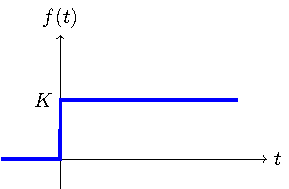
\includegraphics[width=.9\linewidth]{../figs/escalon.pdf}
\end{center}
\end{column}

\begin{column}{0.5\columnwidth}
\[
  f(t) = %
  \begin{cases}
    0 & t < 0\\
    K & t \geq 0
  \end{cases}
  \]
\end{column}
\end{columns}
\end{frame}

\begin{frame}[label={sec:org05d539c}]{Escalón desplazado}
\begin{columns}
\begin{column}{0.5\columnwidth}
\begin{center}
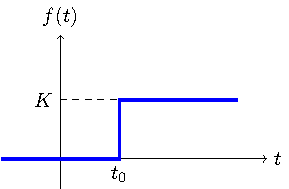
\includegraphics[width=.9\linewidth]{../figs/escalon_t0.pdf}
\end{center}
\end{column}

\begin{column}{0.5\columnwidth}
\[
  f(t) = %
  \begin{cases}
    0 & t < t_0\\
    K & t \geq t_0
  \end{cases}
  \]
\end{column}
\end{columns}
\end{frame}

\begin{frame}[label={sec:orga0082bc}]{Pulso}
\begin{columns}
\begin{column}{0.5\columnwidth}
\begin{center}
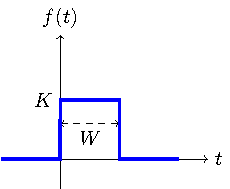
\includegraphics[width=.9\linewidth]{../figs/pulso.pdf}
\end{center}
\end{column}

\begin{column}{0.5\columnwidth}
\[
  f(t) = %
  \begin{cases}
    0 & t < 0\\
    K & 0 \leq t \leq W
  \end{cases}
  \]
\end{column}
\end{columns}
\end{frame}

\begin{frame}[label={sec:orgae1d545}]{Pulso desplazado}
\begin{columns}
\begin{column}{0.5\columnwidth}
\begin{center}
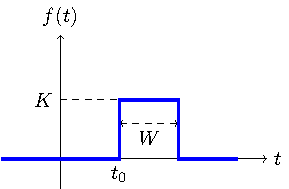
\includegraphics[width=.9\linewidth]{../figs/pulso_t0.pdf}
\end{center}
\end{column}


\begin{column}{0.5\columnwidth}
\[
  f(t) = %
  \begin{cases}
    0 & t < t_0\\
    K & t_0 \leq t \leq t_0 + W
  \end{cases}
  \]
\end{column}
\end{columns}
\end{frame}

\begin{frame}[label={sec:org6180207}]{Rampa}
\begin{columns}
\begin{column}{0.5\columnwidth}
\begin{center}
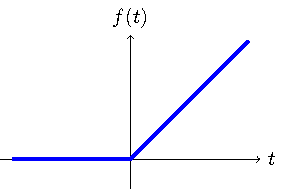
\includegraphics[width=.9\linewidth]{../figs/rampa.pdf}
\end{center}
\end{column}

\begin{column}{0.5\columnwidth}
\[
  f(t) = %
  \begin{cases}
    0 & t < 0\\
    m \cdot t  & t \geq 0
  \end{cases}
  \]
\end{column}
\end{columns}
\end{frame}

\begin{frame}[label={sec:org7f21b03}]{Rampa desplazada}
\begin{columns}
\begin{column}{0.5\columnwidth}
\begin{center}
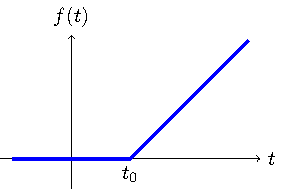
\includegraphics[width=.9\linewidth]{../figs/rampa_t0.pdf}
\end{center}
\end{column}

\begin{column}{0.5\columnwidth}
\[
  f(t) = %
  \begin{cases}
    0 & t < t_0\\
    m \cdot (t - t_0)  & t \geq t_0
  \end{cases}
  \]
\end{column}
\end{columns}
\end{frame}

\begin{frame}[label={sec:orgea90574}]{Triangular}
\begin{columns}
\begin{column}{0.4\columnwidth}
\begin{center}
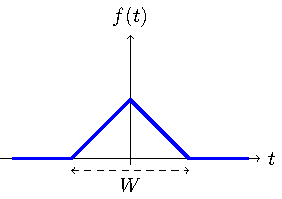
\includegraphics[width=.9\linewidth]{../figs/triangular.pdf}
\end{center}
\end{column}

\begin{column}{0.6\columnwidth}
\[
  f(t) = %
  \begin{cases}
    0 & t < -W/2\\
    m \cdot (t + W/2)  & -W/2 \leq t \leq 0\\
    -m \cdot (t - W/2)  & 0 \leq t \leq W/2\\
    0  & t > W/2
  \end{cases}
  \]
\end{column}
\end{columns}
\end{frame}

\begin{frame}[label={sec:org6cbacbe}]{Triangular desplazada}
\begin{columns}
\begin{column}{0.4\columnwidth}
\begin{center}
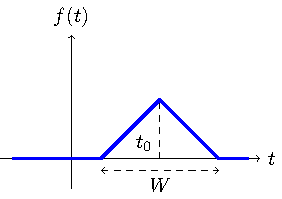
\includegraphics[width=.9\linewidth]{../figs/triangular_t0.pdf}
\end{center}
\end{column}

\begin{column}{0.6\columnwidth}
\[
  f(t) = %
  \begin{cases}
    0 & t < t_0 - W/2\\
    m \cdot [t - (t_0 -  W/2)]  & t_0 - W/2 \leq t \leq t_0\\
    -m \cdot [t - (t_0 + W/2)]  & t_0 \leq t \leq t_0 + W/2\\
    0  & t > t_0 + W/2
  \end{cases}
  \]
\end{column}
\end{columns}
\end{frame}


\section{Teoremas de Linealidad}
\label{sec:orgb5cd630}
\begin{frame}[label={sec:org98452ea}]{Circuitos Lineales}
\begin{itemize}
\item Un circuito eléctrico es lineal si los elementos pasivos y activos que incluye son lineales.
\item Un \alert{elemento pasivo} es lineal si la relación entre la tensión entre sus terminales y la corriente que lo recorre es lineal: \alert{resistencias, condensadores y bobinas}.
\item Una \alert{fuente dependiente} es lineal si su salida (tensión o corriente) tiene una relación lineal con la magnitud del circuito de la que depende.
\item Un circuito lineal tiene dos propiedades:
\begin{itemize}
\item Homogeneidad o \alert{proporcionalidad}.
\item Aditividad o \alert{superposición}.
\end{itemize}
\end{itemize}
\end{frame}

\subsection{Teorema de Proporcionalidad}
\label{sec:org57f9055}

\begin{frame}[label={sec:org858a118}]{Homogeneidad o Proporcionalidad}
Sea \(y(t)\) la respuesta de un \alert{circuito lineal} a una excitación \(x(t)\). 

Si la excitación es multiplicada por una \alert{constante}, \(K \cdot x(t)\), la respuesta del circuito será modificada por la misma constante, \(K \cdot y(t)\).

\begin{center}
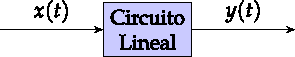
\includegraphics[width=0.6\textwidth]{../figs/proporcionalidad.pdf}
\end{center}
\end{frame}

\begin{frame}[label={sec:org17ebd7b}]{Análisis de un circuito mediante proporcionalidad}
\begin{block}{¿Qué excitación debo aplicar a un circuito para obtener una determinada respuesta?}
\begin{itemize}
\item Aplicamos una excitación de valor unidad.
\item Resolvemos el circuito, obteniendo la respuesta del circuito a la excitación unidad.
\item Hallamos la constante de proporcionalidad entre la respuesta obtenida y la respuesta deseada.
\item La excitación que se debe aplicar es esta constante de proporcionalidad.
\end{itemize}
\end{block}
\end{frame}

\begin{frame}[label={sec:orgee7e0d8}]{Análisis de un circuito mediante proporcionalidad}
\begin{block}{¿Qué respuesta proporciona un circuito ante una determinada excitación?}
\begin{itemize}
\item Suponemos una respuesta de valor unidad.
\item Resolvemos el circuito a la inversa, obteniendo la excitación que provoca la respuesta unidad.
\item Hallamos la constante de proporcionalidad entre la excitación obtenida y la excitación deseada.
\item La respuesta que entrega el circuito es esta constante de proporcionalidad (puede ser un número complejo).
\end{itemize}
\end{block}
\end{frame}

\subsection{Teorema de Superposición}
\label{sec:org7814bc8}

\begin{frame}[label={sec:org08bac37}]{Aditividad o Superposición}
\begin{columns}
\begin{column}{0.5\columnwidth}
La respuesta de un \alert{circuito lineal} a varias fuentes de excitación actuando simultáneamente es igual a la suma de las respuestas que se tendrían cuando actuase cada una de ellas por separado

\[
y(t) = \sum_i y_i(t)
\]
\end{column}

\begin{column}{0.5\columnwidth}
\begin{center}
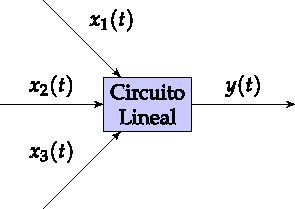
\includegraphics[width=.9\linewidth]{../figs/superposicion.pdf}
\end{center}
\end{column}
\end{columns}
\end{frame}

\begin{frame}[label={sec:org2f5d2d3}]{Análisis de un circuito mediante superposición}
\begin{block}{Procedimiento}
\begin{enumerate}
\item Se apagan todas las fuentes \alert{independientes} del circuito menos una.
\begin{itemize}
\item Las fuentes de tensión se sustituyen por un cortocircuito (\(U = 0\)).
\item Las fuentes de corriente se sustituyen por un circuito abierto (\(I = 0\)).
\item Las fuentes \alert{dependientes} \alert{no} se modifican.
\end{itemize}
\item Se analiza el circuito, obteniendo la respuesta individual a la fuente que permanece activa.
\item Se repite este procedimiento para cada una de las fuentes \alert{independientes} del circuito.
\item La respuesta total del circuito es la suma de las respuestas individuales.
\end{enumerate}
\end{block}
\end{frame}
\begin{frame}[label={sec:org886d7e8}]{Observaciones}
\begin{itemize}
\item \alert{Siempre} hay que aplicar este método cuando en un circuito conviven fuentes de \alert{diferente frecuencia} (o fuentes de corriente continua y corriente alterna).
\item En el caso de fuentes de corriente alterna \alert{sinusoidal}, la respuesta debe expresarse en el \alert{dominio del tiempo}. \alert{No} se pueden \alert{sumar} los \alert{fasores} que corresponden a \alert{frecuencias diferentes}.
\item En el primer paso del procedimiento, se pueden agrupar las fuentes que funcionan a la misma frecuencia y calcular la respuesta del circuito en esa frecuencia.
\end{itemize}
\end{frame}

\begin{frame}[label={sec:org5409c67}]{Potencia}
El principio de superposición aplica a tensiones y corrientes, pero \alert{no} a potencias. Supongamos \(i(t) = i_1(t) + i_2(t)\):
\begin{align*}
  p(t) &= R \cdot i^2(t) =\\
       &= R \cdot (i_1(t) + i_2(t))^2 =\\
       &=R \cdot (i_1^2(t) + i_2^2(t) + 2\cdot i_1(t) \cdot i_2(t))\\
  p(t) &\neq p_1(t) + p_2(t)
\end{align*}
\end{frame}

\begin{frame}[label={sec:org1c30a0f}]{Potencia}
\begin{itemize}
\item Cuando las señales son \alert{ortogonales en un período}\footnote{Dos señales son ortogonales si cumplen la siguiente ecuación:
\[<f_1, f_2>_T = \int_T f_1(t) \cdot f_2(t) dt = 0\]} se pueden sumar las potencias \alert{medias} de cada circuito.
\end{itemize}
\begin{align*}
  P = \sum_i P_i
\end{align*}
\begin{itemize}
\item Ejemplos de señales ortogonales: sinusoidales con diferente frecuencia, una sinusoide con una continua, \ldots{}
\end{itemize}
\end{frame}


\section{Teoremas de Thévenin/Norton}
\label{sec:org1434b9c}

\subsection{Teoremas}
\label{sec:orgdcf8b1a}

\begin{frame}[label={sec:orgaadeb2d}]{Thévenin}
Cualquier \alert{red lineal} compuesta por elementos activos y pasivos puede sustituirse, desde el punto de vista de sus terminales externos AB, por una \alert{fuente de tensión} (generador de Thévenin, \(\epsilon_{th}\)) en \alert{serie} con una impedancia (impedancia de Thévenin, \(Z_{th}\)).

\begin{columns}
\begin{column}{0.5\columnwidth}
\begin{center}
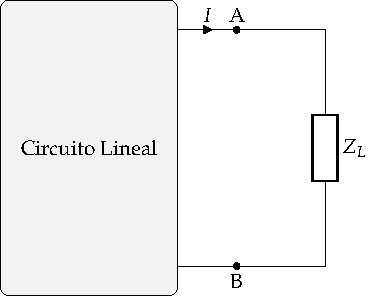
\includegraphics[height=0.6\textheight]{../figs/CircuitoLineal_ZL.pdf}
\end{center}
\end{column}

\begin{column}{0.5\columnwidth}
\begin{center}
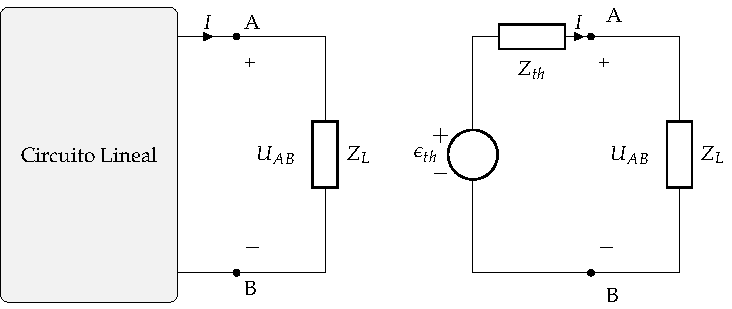
\includegraphics[height=0.6\textheight]{../figs/EquivalenteThevenin.pdf}
\end{center}
\end{column}
\end{columns}
\end{frame}


\begin{frame}[label={sec:org4b4bfd6}]{Norton}
Cualquier \alert{red lineal} compuesta por elementos activos y pasivos puede sustituirse, desde el punto de vista de sus terminales externos AB, por una \alert{fuente de corriente} (generador de Norton, \(I_N\)) en \alert{paralelo} con una impedancia (impedancia de Norton, \(Z_N\)).

\begin{columns}
\begin{column}{0.5\columnwidth}
\begin{center}
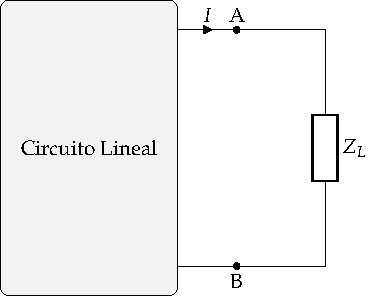
\includegraphics[height=0.6\textheight]{../figs/CircuitoLineal_ZL.pdf}
\end{center}
\end{column}

\begin{column}{0.5\columnwidth}
\begin{center}
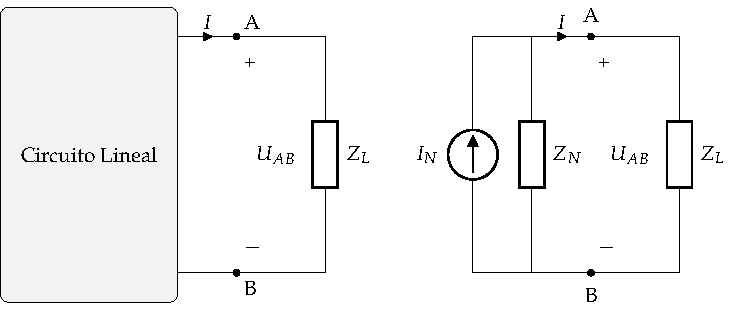
\includegraphics[height=0.6\textheight]{../figs/EquivalenteNorton.pdf}
\end{center}
\end{column}
\end{columns}
\end{frame}

\subsection{Cálculo}
\label{sec:orgaa48b35}
\begin{frame}[label={sec:org1551971}]{Cálculo del equivalente de Thévenin}
\begin{columns}
\begin{column}{0.5\columnwidth}
\begin{center}
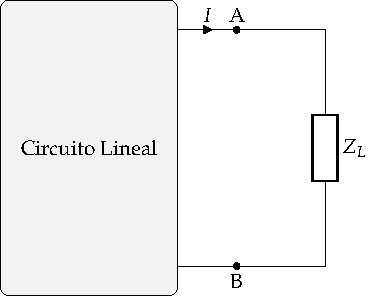
\includegraphics[height=0.38\textheight]{../figs/CircuitoLineal_ZL.pdf}
\end{center}
\end{column}

\begin{column}{0.5\columnwidth}
\begin{center}
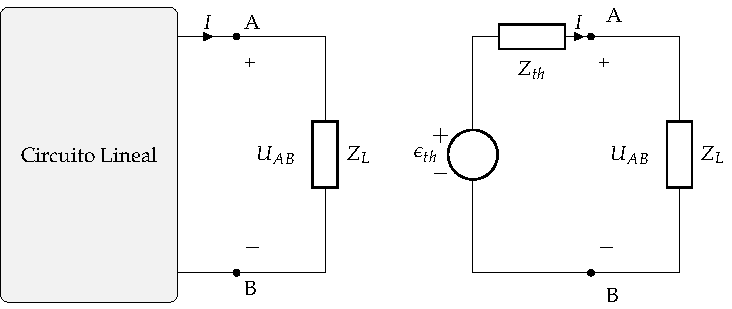
\includegraphics[height=0.38\textheight]{../figs/EquivalenteThevenin.pdf}
\end{center}
\end{column}
\end{columns}


\begin{itemize}
\item Circuito Abierto (\(Z_L \to \infty, \quad U_{AB} = U_{oc}\))
\end{itemize}
\[
\boxed{\epsilon_{th} = U_{oc}}
\]
\begin{itemize}
\item Cortocircuito (\(Z_L = 0, \quad I = I_{sc}\))
\end{itemize}
\[
\boxed{Z_{th} = \frac{\epsilon_{th}}{I_{sc}} = \frac{U_{oc}}{I_{sc}}}
\]
\end{frame}

\begin{frame}[label={sec:orgb8d7433}]{Cálculo del equivalente de Norton}
\begin{columns}
\begin{column}{0.5\columnwidth}
\begin{center}
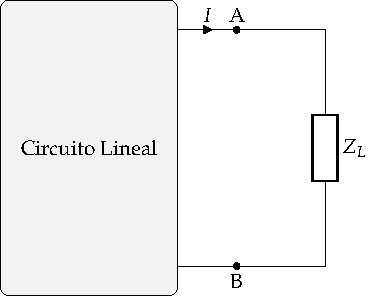
\includegraphics[height=0.38\textheight]{../figs/CircuitoLineal_ZL.pdf}
\end{center}
\end{column}

\begin{column}{0.5\columnwidth}
\begin{center}
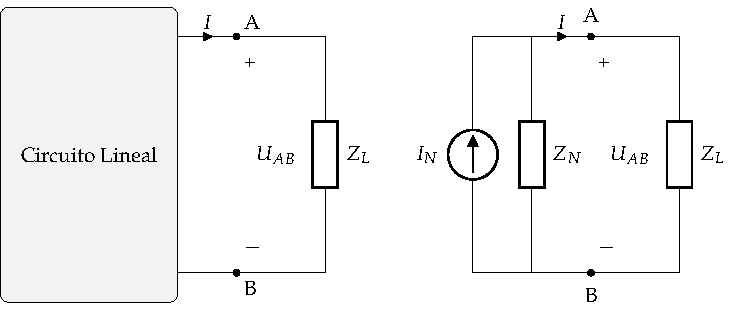
\includegraphics[height=0.38\textheight]{../figs/EquivalenteNorton.pdf}
\end{center}
\end{column}
\end{columns}

\begin{itemize}
\item Cortocircuito (\(Z_L = 0, \quad I = I_{sc}\))
\end{itemize}
\[
\boxed{I_N = I_{sc}}
\]
\begin{itemize}
\item Circuito Abierto (\(Z_L \to \infty, \quad U_{AB} = U_{oc}\))
\end{itemize}
\[
\boxed{Z_N = \frac{U_{oc}}{I_N} = \frac{U_{oc}}{I_{sc}}}
\]
\end{frame}

\begin{frame}[label={sec:org0b88b88}]{Observaciones}
\begin{itemize}
\item Cálculo de la impedancia:
\begin{itemize}
\item Si el circuito \alert{no} contiene fuentes dependientes, se puede realizar \alert{apagando} todos los \alert{generadores} y obteniendo la impedancia equivalente.
\item Si el circuito contiene fuentes dependientes, es necesario conectar un \alert{generador de prueba} a la salida del circuito y obtener la relación entre la tensión y corriente de este generador.
\end{itemize}

\item Gracias a la equivalencia de fuentes, una vez obtenido uno de los equivalentes se puede obtener el otro mediante una transformación.
\end{itemize}
\end{frame}
\begin{frame}[label={sec:org3fd0a49}]{Recordatorio: equivalencia de fuentes}
Sólo es posible establecer equivalencia entre \alert{fuentes reales}.
\begin{columns}
\begin{column}{0.33\columnwidth}
\begin{center}
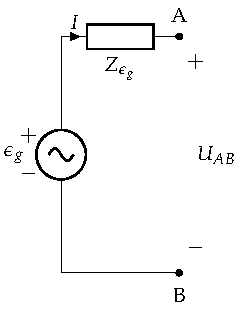
\includegraphics[height=0.5\textheight]{../figs/FuenteTensionReal.pdf}
\end{center}
\[
  \overline{U}_{AB} = \overline{\epsilon}_g - \overline{Z}_{\epsilon_g} \cdot \overline{I}
\]
\end{column}
\begin{column}{0.33\columnwidth}
\begin{align*}
  \overline{Z}_g &= \overline{Z}_{\epsilon_g} = \overline{Z}_{I_g}\\
  \overline{\epsilon}_g &= \overline{Z}_g \cdot \overline{I}_g\\
  \overline{I}_g &= \frac{\overline{\epsilon}_g}{\overline{Z}_g}
\end{align*}
\end{column}
\begin{column}{0.33\columnwidth}
\begin{center}
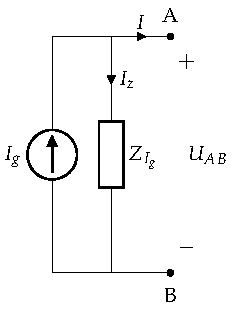
\includegraphics[height=0.5\textheight]{../figs/FuenteCorrienteReal.pdf}
\end{center}
\[
  \overline{I} = \overline{I}_g - \frac{\overline{U}_{AB}}{\overline{Z}_{I_g}}
\]
\end{column}
\end{columns}
\end{frame}


\section{Teorema de máxima transferencia de potencia}
\label{sec:org9ab4cea}

\begin{frame}[label={sec:orgd815c4c}]{Planteamiento}
Sea el circuito lineal de la figura. ¿Qué impedancia \(Z_L\) hay que conectar en los terminales AB para que el circuito entregue la máxima potencia disponible?

\begin{center}
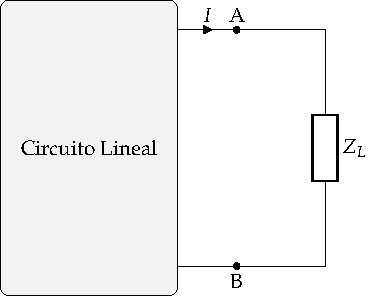
\includegraphics[height=0.55\textheight]{../figs/CircuitoLineal_ZL.pdf}
\end{center}

Resolvemos esta pregunta mediante el generador equivalente de Thévenin.
\end{frame}


\subsection{Cálculo}
\label{sec:org660eb18}
\begin{frame}[label={sec:org6825aa2}]{Ecuaciones}
Calculamos la potencia activa en la impedancia de carga \(Z_L\):
\begin{columns}
\begin{column}{0.3\columnwidth}
\begin{center}
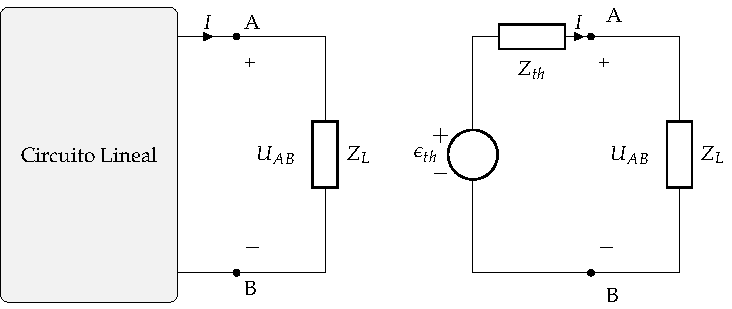
\includegraphics[height=0.45\textheight]{../figs/EquivalenteThevenin.pdf}
\end{center}
\end{column}

\begin{column}{0.2\columnwidth}
\begin{align*}
  \overline{Z}_{th} &= R_{th} + jX_{th}\\
  \overline{Z}_L &= R_L + jX_L\\
\end{align*}
\end{column}

\begin{column}{0.4\columnwidth}
\begin{align*}
\overline{I} &= \frac{\overline{\epsilon}_{th}}{\overline{Z}_{th} + \overline{Z}_L}\\
P_L &= I^2 \cdot R_L\\
\Aboxed{P_L &= \frac{\epsilon^2_{th}}{|\overline{Z}_{th} + \overline{Z}_L|^2} \cdot R_L}
\end{align*}
\end{column}
\end{columns}

Las condiciones de máximo son: 
\[
  \boxed{%
    \diffp{P_L}{X_L} = 0 \quad%
    \diffp{P_L}{R_L} = 0%
  }
\]
\end{frame}

\begin{frame}[label={sec:org4c919d9}]{Reactancia}
A partir de la expresión de potencia en la carga\ldots{}
\[
  P_L = \frac{\epsilon^2_{th}}{|\overline{Z}_{th} + \overline{Z}_L|^2} \cdot R_L
\]
calculamos la derivada parcial respecto de la reactancia:
\[
  \diffp{P_L}{X_L} = \epsilon^2_{th} \cdot R_L \cdot \left[\frac{-1}{\left((R_L + R_{th})^2 + (X_L + X_{th})^2\right)^2} \cdot 2 \cdot (X_L + X_{th})\right]
\]
Aplicamos la condición de máximo y obtenemos un resultado parcial:
\[
   \diffp{P_L}{X_L} = 0 \Rightarrow \boxed{X_L = - X_{th}}
\]
\end{frame}

\begin{frame}[label={sec:org094e0f8}]{Resistencia}
Simplificamos la expresión de la potencia teniendo en cuenta el resultado anterior (\(X_L = - X_{th}\)):
\[
  P_L = \frac{\epsilon^2_{th}}{(R_{th} + R_L)^2} \cdot R_L
\]
Calculamos la derivada parcial respecto de la resistencia:
\begin{align*}
  \diffp{P_L}{R_L} &= \epsilon^2_{th} \cdot \left[\frac{1}{(R_L + R_{th})^2} - 2 \cdot \frac{R_L}{(R_L + R_{th})^3}\right]\\
		   &= \frac{\epsilon^2_{th} \cdot (R_{th} - R_L)}{(R_L + R_{th})^3}
\end{align*}
Nuevamente, aplicamos la condición de máximo y obtenemos la resistencia:
\[
   \diffp{P_L}{R_L} = 0 \Rightarrow \boxed{R_L = R_{th}}
\]
\end{frame}


\subsection{Impedancia y Potencia}
\label{sec:org1632c15}

\begin{frame}[label={sec:orgbdd03f1}]{Impedancia de Carga}
Dado un circuito lineal (del que podemos calcular su equivalente de Thévenin) \ldots{}
\begin{center}
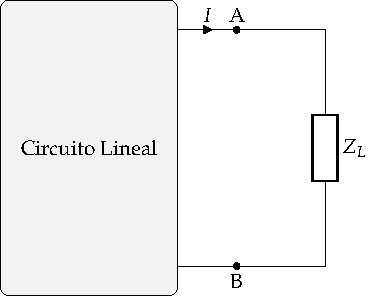
\includegraphics[height=0.45\textheight]{../figs/CircuitoLineal_ZL.pdf}
\end{center}

\ldots{} la impedancia de carga que hay que conectar entre sus terminales AB para obtener la máxima potencia disponible es:
\[
  \boxed{\overline{Z}_L = \overline{Z}_{th}^*}
\]
\end{frame}

\begin{frame}[label={sec:org5c45c0d}]{Máxima potencia disponible}
La máxima potencia disponible en la carga es:
\begin{center}
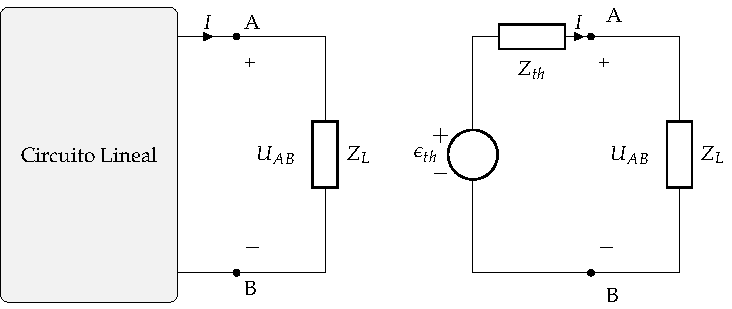
\includegraphics[height=0.45\textheight]{../figs/EquivalenteThevenin.pdf}
\end{center}

\begin{equation*}
  \left.
    \begin{matrix}
      \overline{Z}_L = \overline{Z}_{th}^*\\
      P_L = \frac{\epsilon^2_{th}}{|\overline{Z}_{th} + \overline{Z}_L|^2} \cdot R_L
    \end{matrix} \right\}\rightarrow
  \boxed{P_L = \frac{\epsilon^2_{th}}{4 R_{th}}}
\end{equation*}
\end{frame}
\end{document}
